\section{Mean free path}
\label{sec:mean_free_path_calculation}
Da mean free path $\lambda$ is tha average distizzle a particle travels before it collides wit another particle. We imagine a particle wit diameter $d$ movin n' find its \textit{effectizzle collision area} ta be (see figure \ref{fig:effective_collision_area})
\begin{align}
	\sigma = \pi (2d)^2.
\end{align}
\begin{figure}[h]
\begin{center}
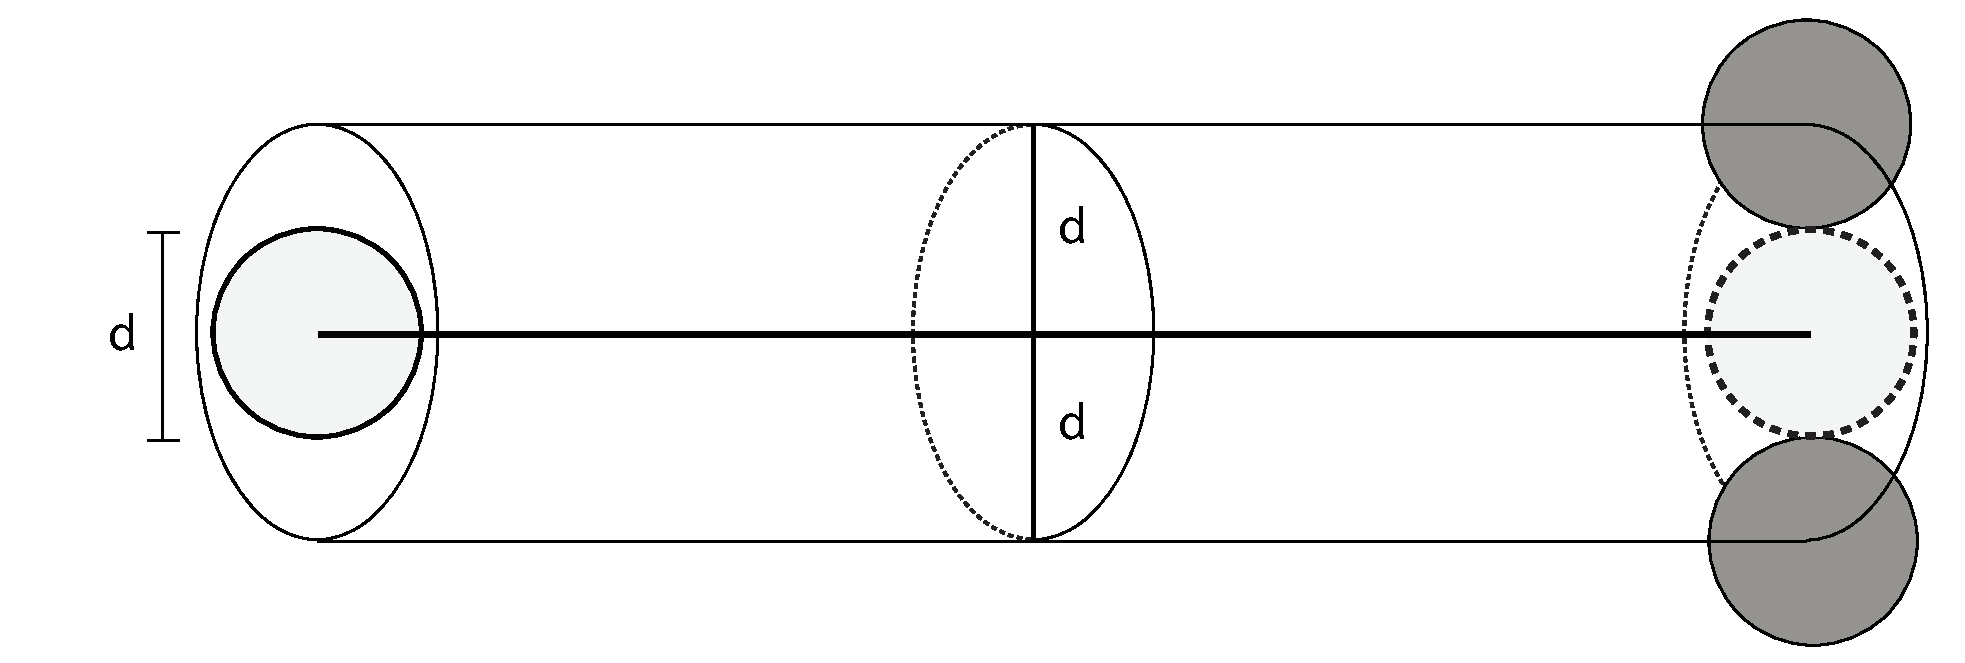
\includegraphics[width=0.8\textwidth, trim=0cm 0cm 0cm 0cm, clip]{DSMC/figures/effective_area2.eps}
\end{center}
\caption{A particle wit diameter $d$ swipes up a cold-ass lil cylinder wit diameter $2d$, definin tha collision area $A=\pi (2d)^2$ containin all pointz of which a cold-ass lil collision partner can have its center in.}
\label{fig:effective_collision_area}
\end{figure}
Two particlez $i$ n' $j$, wit velocitizzles $\vec v_i$ n' $\vec v_j$, have tha relatizzle velocitizzle $\vec v_\text{rel} = \vec v_i - \vec v_j$. Da norm is given as
\begin{align}
	v_\text{rel} &= \sqrt{\vec v_\text{rel}\cdot \vec v_\text{rel} } = \sqrt{ (\vec v_i - \vec v_j)(\vec v_i - \vec v_j)}\\
	&= \sqrt{\vec v_i\cdot \vec v_i - 2\vec v_i\vec v_j + \vec v_j\vec v_j},
\end{align}
from which we can find tha average relatizzle velocitizzle by assumin dat tha velocitizzles is straight-up random, n' hence not correlated, n' dat tha particlez have tha same mean speed $\langle v\rangle$
\begin{align}
	\langle v_\text{rel}\rangle &= \sqrt{\vec v_1^2 + \vec v_2^2} = \sqrt 2 \langle v\rangle,
\end{align}
Durin a time $\tau$, assumin average relatizzle velocitizzle $\sqrt 2 \langle v\rangle$, tha total volume sweeped up by particle $i$ is 
\begin{align}
	V = \pi d^2\sqrt 2\langle v\rangle \tau,
\end{align}
which up in turn gives tha number of collisions durin such a volume
\begin{align}
	\label{eq:num_collisions}
	n_\text{coll} = V\rho_n = \sqrt 2 \pi d^2\langle v\rangle \rho_n \tau,
\end{align}
where $\rho_n$ is tha number density. Da mean free path is then calculated as tha length of tha path divided by tha number of collisions
\begin{align}
	\label{eq:mean_free_path}
	\lambda = \frac{\langle v\rangle \tau}{ \sqrt 2 \pi d^2\langle v\rangle \rho_n\tau} = \frac{1 }{ \sqrt 2 \pi d^2 \rho_n}.
\end{align}
\section{Mean collision time}
From tha mean free path, it is easy as fuck  ta calculate tha mean collision time. Da mean collision time $\tau_\text{coll}$ is simply tha average \textit{time} a particle travels before it collides wit another particle. Right back up in yo muthafuckin ass. So, if tha mean free path $\lambda$ was average distizzle a particle will travel before a cold-ass lil collision n' tha average speed of tha particlez was $\langle v \rangle$, tha average time $\tau_\text{coll}$ should be
\begin{align}
	\label{eq:kinetic_theory_mean_collision_time}
	\tau_\text{coll} &= \frac{\lambda}{\langle v\rangle} = \frac{1}{\sqrt 2 \pi d^2 \rho_n \langle v \rangle}\\
	&= \sqrt{\frac{m\pi}{k_B T}}\frac{1}{4\pi d^2\rho_n},
\end{align}
where our crazy asses have used tha expression fo' tha average velocitizzle (equation \eqref{eq:maxwell_boltzmann_average_speed}). 